\section{Invariant solutions}

Invariant structures, together with their stable and unstable
manifolds, shape the geometrical structure of the
\statesp. We also anticipate that \spt\ averages can be
calculated by \po s, as discussed in \refsect{sec:det}.
Since invariant structures play such an important role in chaotic systems,
we now discuss them in the one\dmn\
\KSe\ with $L=22$. These include \eqva, \reqva, pre\po s, and
\rpo s, whose definitions can be found in \refsect{sec:cred}.

\subsection{\Eqva\ and \reqva}

There are only three \eqva\ and two \reqva\ for domain size $L = 22$\rf{SCD07}.
They can be obtained by Newton-based numerical search such as
the Levenberg-Marquardt algorithm\rf{levenberg44, Marquardt63}
even with random initial inputs.

\begin{figure}[h]
  \centering
  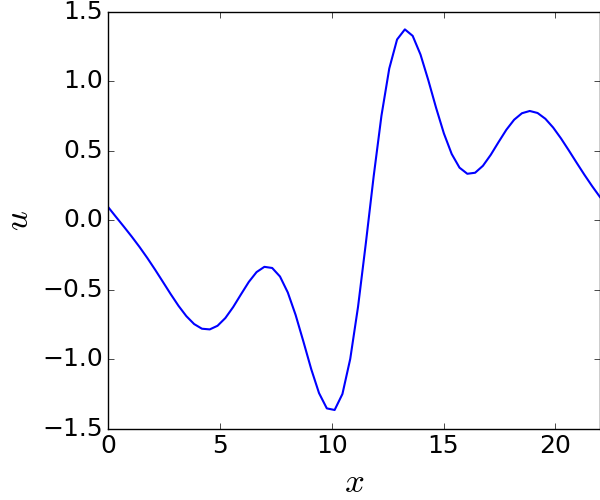
\includegraphics[width=0.32\textwidth]{ksEq1}
  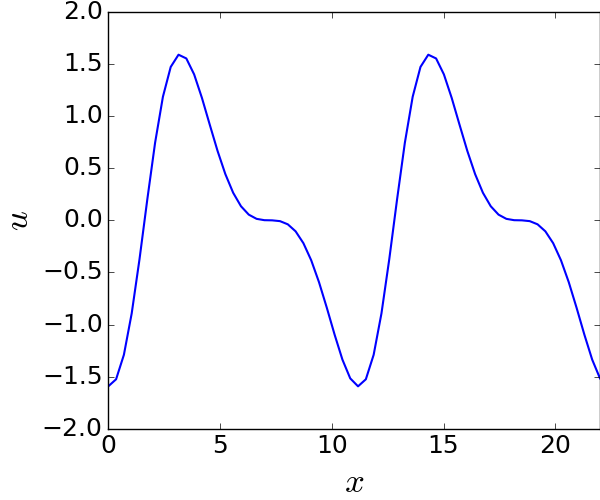
\includegraphics[width=0.32\textwidth]{ksEq2}
  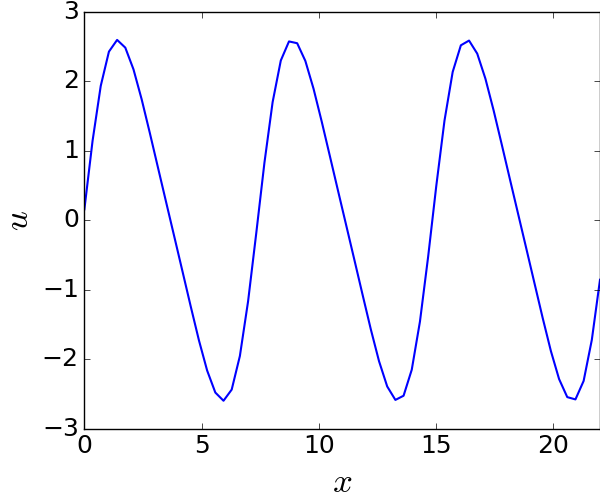
\includegraphics[width=0.32\textwidth]{ksEq3}
  \caption[Three \eqva\ in the one\dmn\ \KSe.]
  {
    Three \eqva\ \EQV{1}, \EQV{2}, and \EQV{3} from left to right in the one\dmn\ \KSe.
  }
  \label{fig:kseq}
\end{figure}

\refFig{fig:kseq} shows the profiles of these three \eqva. \EQV{1} is in
the anti-symmetric subspace $\ssp(x, t) = -\ssp(-x, t)$. \EQV{2} and
\EQV{3} are period-2 and period-3 harmonic solutions. Since $a_1 = 0$,
\EQV{2} and \EQV{3} are in the slice border.

\begin{figure}[h]
  \centering
  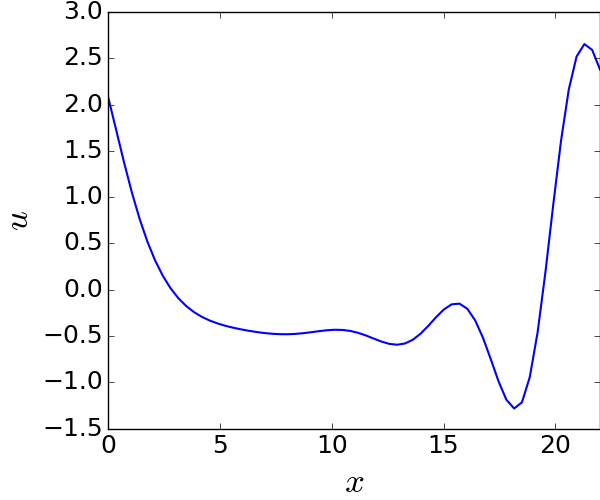
\includegraphics[width=0.45\textwidth]{ksReq1}
  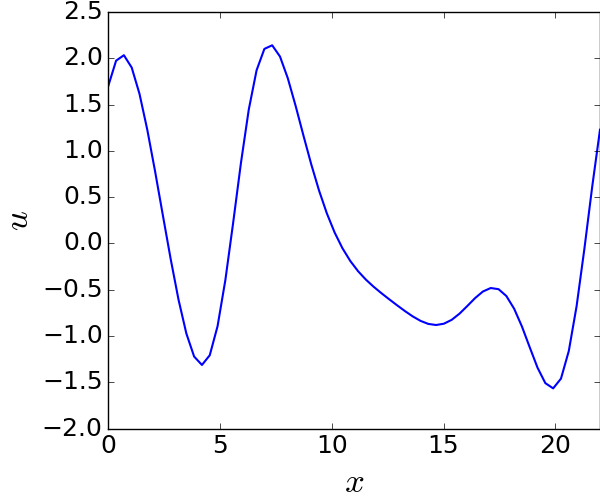
\includegraphics[width=0.45\textwidth]{ksReq2}
  \caption[Two \Reqva\ in the one\dmn\ \KSe.]
  {
    Two \reqva\ \REQV{1}{} (left) and \REQV{2}{}
    (right) in the one\dmn\ \KSe.
  }
  \label{fig:ksreq}
\end{figure}

\begin{figure}[h]
  \centering
  (a)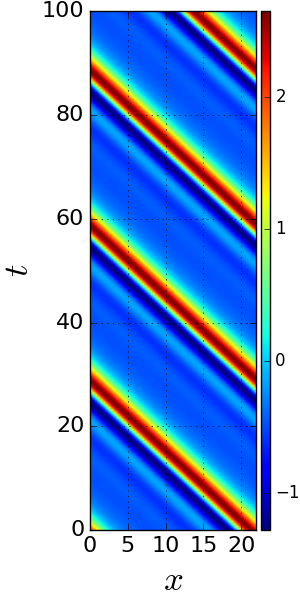
\includegraphics[width=0.2\textwidth]{ksReq1T100}
  (b)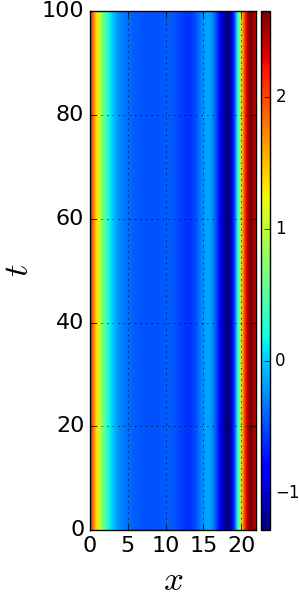
\includegraphics[width=0.2\textwidth]{ksReq1T100Red}
  (c)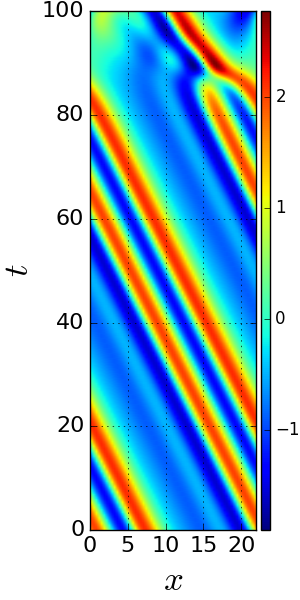
\includegraphics[width=0.2\textwidth]{ksReq2T100}
  (d)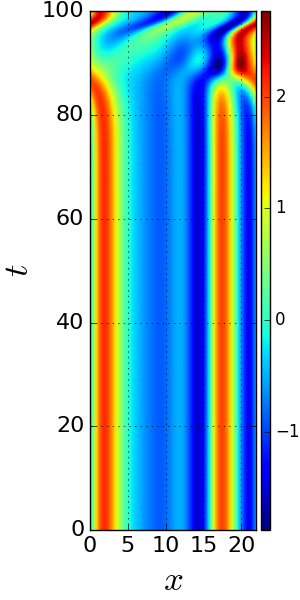
\includegraphics[width=0.2\textwidth]{ksReq2T100Red}
  \caption[\Reqva\ in the full \statesp\ and in the slice in the one\dmn\ \KSe.]
  {
    (a)(c) \REQV{1}{} and \REQV{2}{} in the full \statesp.
    (b)(d) \REQV{1}{} and \REQV{2}{} in the slice.
  }
  \label{fig:ksreqT100}
\end{figure}

\refFig{fig:ksreq} shows the profiles of the two \reqva. Their time-evolution profiles
are shown in \reffig{fig:ksreqT100}(a)(c). The color of the heat map represents $u(x, t)$.
Both of them have constant spatial translation velocity. That is why they are also called
\emph{traveling waves}. The in-slice trajectories are shown in \reffig{fig:ksreqT100}(b)(d),
in which translation symmetry has been reduced. Note, \REQV{2}{} fails to maintain its
profile after $t=80$ due to its instability. For the stability exponents of these three
\eqva\ and two
\reqva, please see\rf{SCD07}.

\subsection{Pre\po s and \rpo s}

\begin{figure}[ht]
  \centering
  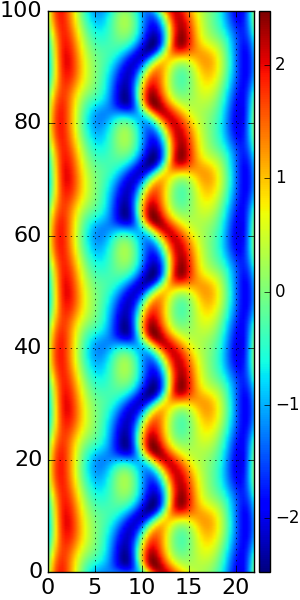
\includegraphics[width=0.16\textwidth]{ksppo1T100NoLabel}
  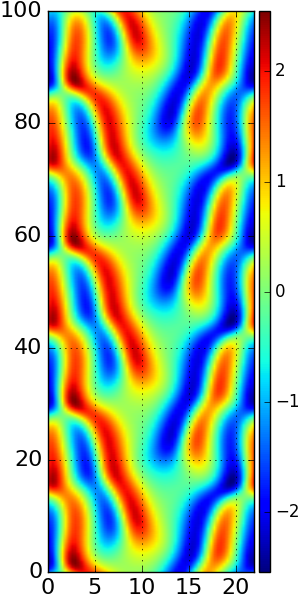
\includegraphics[width=0.16\textwidth]{ksppo2T100NoLabel}
  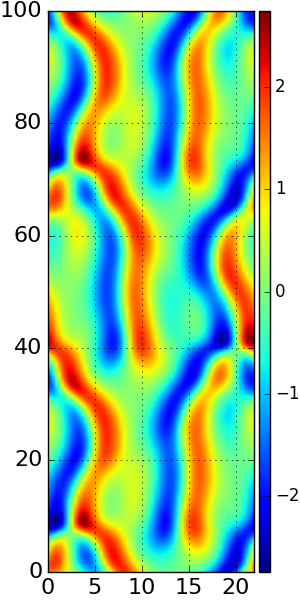
\includegraphics[width=0.16\textwidth]{ksppo3T100NoLabel}
  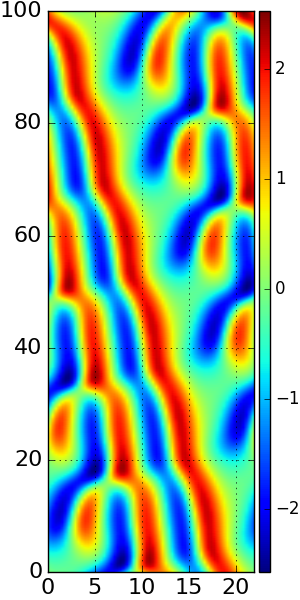
\includegraphics[width=0.16\textwidth]{ksrpo1T100NoLabel}
  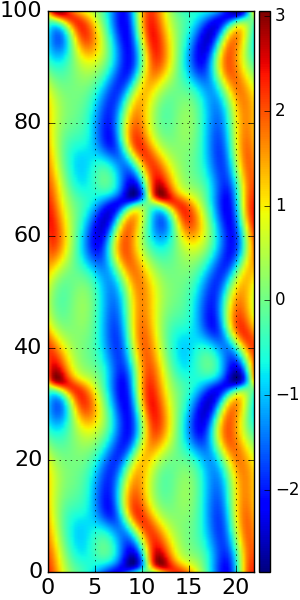
\includegraphics[width=0.16\textwidth]{ksrpo2T100NoLabel}
  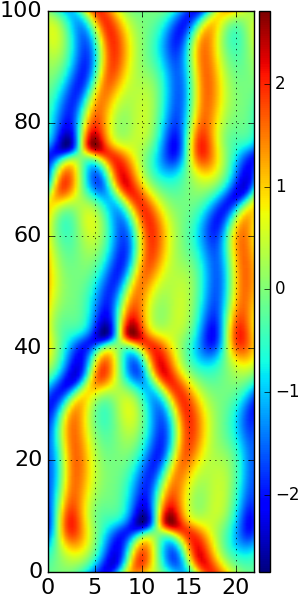
\includegraphics[width=0.16\textwidth]{ksrpo3T100NoLabel}
  \caption[Pre\po s and \rpo s in the full \statesp.]
  {
    The shortest three pre\po s and three \rpo s in the full \statesp.
    Left three: \PPO{10.25}, \PPO{14.33} and \PPO{32.36}.
    Right three: \RPO{16.31}, \RPO{32.80} and \RPO{33.50}.
  }
  \label{fig:kspoT100}
\end{figure}

\begin{figure}[ht]
  \centering
  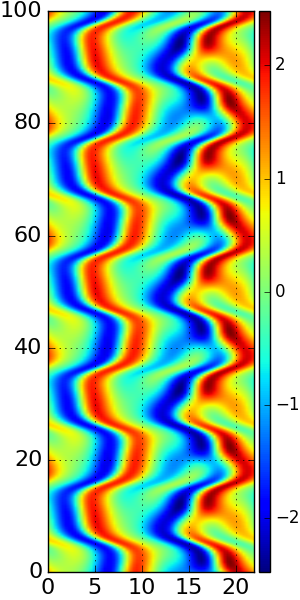
\includegraphics[width=0.16\textwidth]{ksppo1T100NoLabelRed}
  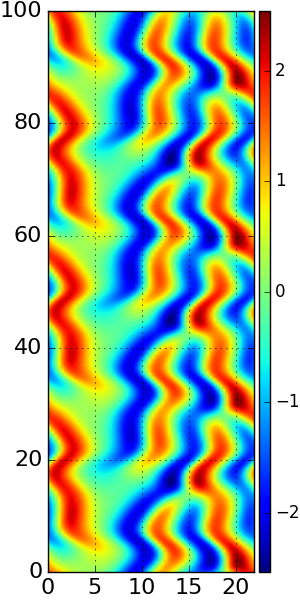
\includegraphics[width=0.16\textwidth]{ksppo2T100NoLabelRed}
  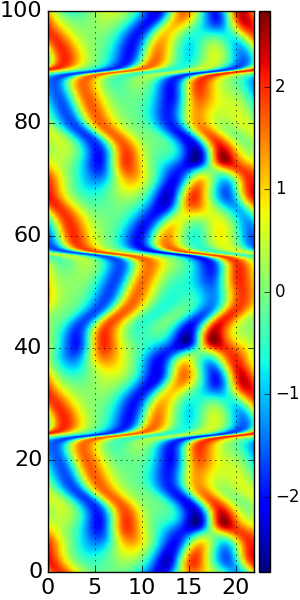
\includegraphics[width=0.16\textwidth]{ksppo3T100NoLabelRed}
  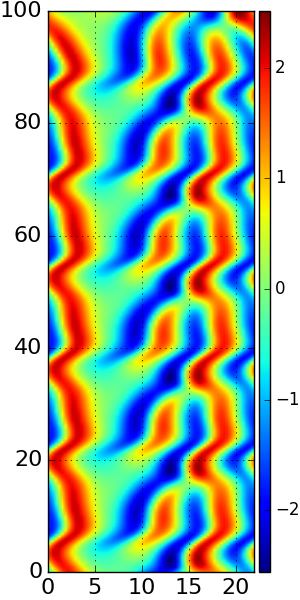
\includegraphics[width=0.16\textwidth]{ksrpo1T100NoLabelRed}
  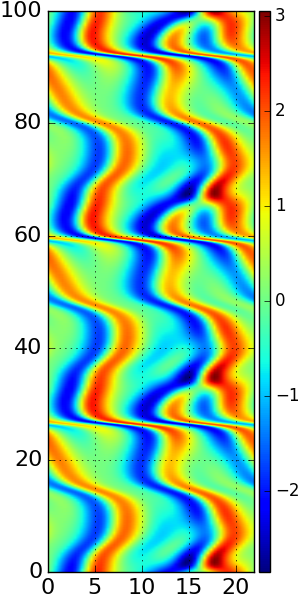
\includegraphics[width=0.16\textwidth]{ksrpo2T100NoLabelRed}
  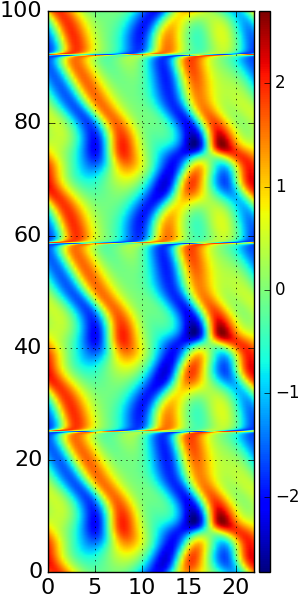
\includegraphics[width=0.16\textwidth]{ksrpo3T100NoLabelRed}
  \caption[Pre\po s and \rpo s in the slice.]
  {Orbits of \reffig{fig:kspoT100} in the slice.}
  \label{fig:kspoT100Red}
\end{figure}

Using a multishooting method, over $60\,000$ pre\po s and \rpo s\rf{SCD07} are found with
periods ranging from $10.25$ to $200$. All of them have either one or two
unstable directions. Let \PPO{T} and \RPO{T} denote the pre\po\ and \rpo\ with
period $T$ respectively. \refFig{fig:kspoT100} shows the shortest three pre\po s and
shortest three \rpo s. A pre\po\ reflects itself after one prime period, so it is
truly periodic after two prime periods. While a \rpo\ has a specific
spatial translation after each period. \refFig{fig:kspoT100Red} shows the
corresponding in-slice orbits. Since translation symmetry has been reduced,
\rpo s become periodic in the slice. Note, some of them undergo quick twists
at certain times. This is because we are using a post-processing method to transform
orbits in the full \statesp\ to the slice; therefore, when an orbit
gets close to the slice border, the rotation phase jumps sharply. If we integrate
the system directly in the slice by \refeq{eq:ksRescale}, then time will dilate when
an orbit gets close to the slice border.

\begin{table}[!ht]
  %\footnotesize
  \caption[Floquet exponents of pre\po s and \rpo s.]{
    The first 10 and last four Floquet multipliers
    $ \ExpaEig_i= \exp(\period{}\,\eigRe[i] \pm i\theta_{i})$ for
    six representative orbits.
    $\theta_{i}$ column lists either the phase,
    if the Floquet multiplier is complex, or `-1' if the
    multiplier is real, but inverse hyperbolic.
  }
  \label{tab:floquet_ppo1}
  \centering
  \begin{tabular}{l l c | l l c | l l c}
    \hline
    \multicolumn{3}{c |}{\PPO{10.25}} & \multicolumn{3}{c |}{\PPO{14.33}} & \multicolumn{3}{c}{\PPO{32.36}} \\
    \hline
    $i$ & ~~~~~$\eigRe[i]$  & $\theta_{i}$  & $i$ & ~~~~~$\eigRe[i]$ & $\theta_{i}$  & $i$ & ~~~~~$\eigRe[i]$  & $\theta_{i}$ \\
    \hline
    1,2 & ~0.033209  &    $\pm$2.0079  &     1 &          0.31095    &   -1               &     1,2&           0.064755   &  $\pm$1.9790       \\
    3 & -4.1096e-13  &                 &     2 &         -1.7825e-12 &                    &      3 &          -6.3772e-14 &                    \\
    4 & -3.3524e-14  &    -1           &     3 &          2.5049e-13 &   -1               &      4 &           1.9306e-13 &  -1                \\
    5 &  -0.21637    &                 &     4 &         -0.12154    &   -1               &      5 &          -0.17511    &                    \\
    6,7 &  -0.26524  &   $\pm$2.6205   &     5 &         -0.20150    &                    &      6 &          -0.24418    &  1                 \\
    8 &  -0.33073    &    -1           &     6 &         -0.29265    &   -1               &     7,8&          -0.27968    &  $\pm$0.6990       \\
    9 &  -1.9605    &                  &     7,8 &       -0.34313    &    $\pm$1.7872     &      9 &          -1.9868     &  -1                \\
    10 & -1.9676    &    -1            &     9 &         -1.9530    &   -1                &     10 &         -1.9891      &                    \\
       &            &                  &     10 &        -1.9928    &                     &        &                      &                    \\
       &  $\cdots$  &                  &       &         $\cdots$  &                      &        &           $\cdots$   &                    \\
    59 &  -5313.6   &    -1           &     59 &         -5312.7   &   -1                 &     59 &          -5313.3     &  -1                \\
    60 &  -5317.6   &                 &     60 &         -5318.4   &                      &     60 &          -5317.9     &                    \\
    61 &  -6051.8   &    -1           &     61 &         -6057.8   &                      &     61 &          -6052.9     &                    \\
    62 &  -6080.4   &                 &     62 &         -6074.4   &   -1                 &     62 &          -6079.2     &  -1                \\
    \hline \hline
    \multicolumn{3}{c |}{\RPO{16.31}} & \multicolumn{3}{c |}{\RPO{32.80}} & \multicolumn{3}{c}{\RPO{33.50}} \\
    \hline
    $i$ & ~~~~~$\eigRe[i]$  & $\theta_{i}$  & $i$ & ~~~~~$\eigRe[i]$ & $\theta_{i}$  & $i$ & ~~~~~$\eigRe[i]$  & $\theta_{i}$ \\
    \hline
    1 &     ~0.32791  &                  &  1,2 &      0.018610    &     $\pm$1.397964    & 1   &     0.073049   &                      \\
    2 &   ~2.8679e-12  &                 &  3   &      6.1717e-14  &                      & 2   &     0.015160   &   -1                 \\
    3 &   ~2.3559e-13  &                 &  4   &      -5.7430e-14 &                      & 3   &     1.1725e-14 &                      \\
    4 &     -0.13214  &        -1        &  5   &      -0.19688    &    -1                & 4   &    -8.8541e-14 &                      \\
    5,6 &   -0.28597  & $\pm$2.7724      &  6   &        -0.24726  &    -1                & 5   &    -0.11390    &   -1                 \\
    7 &     -0.32821  &       -1         &  7,8 &        -0.30869  &     $\pm$2.20628     & 6   &    -0.25224    &                      \\
    8 &      -0.36241  &                 &  9   &         -1.9660  &    -1                & 7,8 &    -0.26398    &   $\pm$1.0521        \\
    9,10 &   -1.9617  &  $\pm$2.2411     &  10  &         -1.9575  &    -1                & 9,10&    -1.993196   &   $\pm$0.60493       \\
         &  $\cdots$ &                   &      &         $\cdots$ &                      &     &     $\cdots$   &                      \\
    59 &   -5314.4 &                     &  59  &         -5313.9  &                      & 59  &    -5313.2     &  -1                  \\
    60 &   -5317.7 &                     &  60  &         -5317.2  &                      & 60  &    -5318.0     &  -1                  \\
    61 &   -6059.2 &                     &  61  &         -6053.9  &    -1                & 61  &    -6052.5     &                      \\
    62 &   -6072.9 &                     &  62  &         -6078.3  &    -1                & 62  &    -6079.7     &                      \\
    \hline
  \end{tabular}
\end{table}

\begin{figure}[ht]
  \centering
  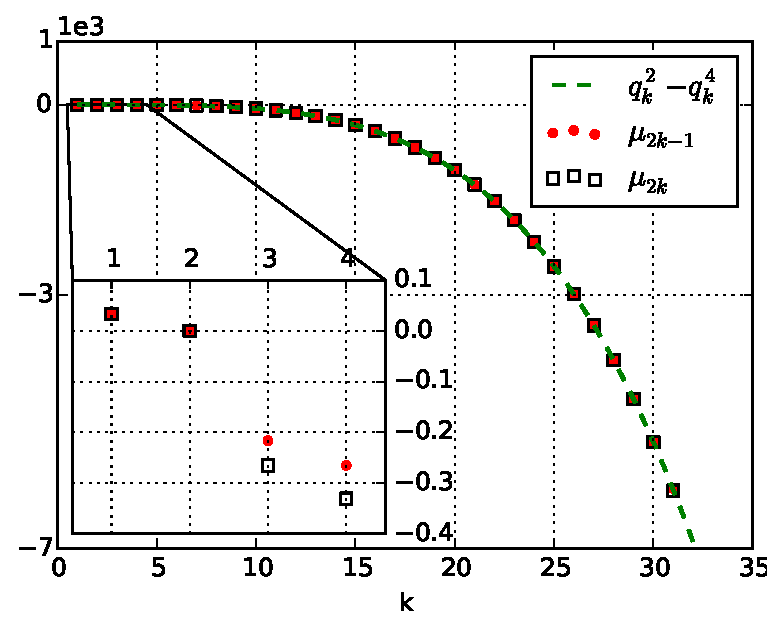
\includegraphics[width=0.6\textwidth]{ppo1spectrum64}
  \caption[Floquet spectrum of \PPO{10.25}.]{
    The real parts of the Floquet exponents paired for a given $k$ as
    $(k,\eigRe[2k-1])$ and $(k,\eigRe[2k])$ for \PPO{10.25}.
    The dashed line (green) is
    $q_{k}^{2}-q_{k}^{4}$ with $q_k = 2\pi k/L$.
    The inset is a magnification of the region
    containing the 8 leading exponents.
  }
  \label{fig:ppo1spect}
\end{figure}

This set of preperodic or relative \po s forms the backbone of the global attractor. An ergodic
trajectory shadows one orbit for a certain period and then is repelled to the neighborhood of
another orbit. This random walk is determined by the stability of the preperodic and relative
\po s.
\refTab{tab:floquet_ppo1} gives the Floquet exponents of the six orbits in \reffig{fig:kspoT100},
which are obtained by \ped\ algorithm that will be covered in \refchap{chap:ped}.
There are a few observations. First, all orbits have one or two unstable directions and
are weakly unstable. \PPO{14.33} and \RPO{16.31} are the two most unstable orbits
in our database.
% Actually, these two orbits shadow each other in the symmetry reduced
% \statesp, which will be shown in \refsect{sect:shadow}.
Second, all orbits have
two marginal directions. For pre\po s, one marginal direction has inverse hyperbolicity, \ie,
one Floquet multiplier is equal to $-1$. This was proved in \refexam{exam:KSmarginal}.
Third, the leading 8 Floquet exponents vary sharply among different orbits, but the remaining
spectrum is similar. More precisely, for large index $k$, the real parts of
Floquet exponents lie
on the curve $(q_k^2 - q_k^4 )$ as shown in \reffig{fig:ppo1spect} for \PPO{10.25}.
This means that the nonlinear term in \refeq{eq:ksfourier} is almost negligible for higher
Fourier modes, and thus they are decoupled from other modes and shrink exponentially with
rate $|q_k^2 - q_k^4 |$.
Also, Floquet exponents appear in pairs for large indices simply because
the real and complex part of high Fourier modes have a similar contraction
rate.
From these observations, we gain an intuition of how many directions
are important in shaping the neighborhood of a pre/relative \po.
